\documentclass[12pt]{article}
\usepackage{amsmath,amssymb,amsthm}
\usepackage{graphicx,mathabx}
\usepackage{xcolor}
\usepackage{tikz}
\usepackage{placeins}
\usepackage{lipsum}
\usepackage{mathtools}
\usepackage[shortlabels]{enumitem}
\usepackage{wrapfig}
\DeclarePairedDelimiter{\ceil}{\lceil}{\rceil}
\begin{document}
\title{TCSS 343 - Week 2 - Thursday}
\author{Jake McKenzie}
\maketitle
\noindent\centerline{\textbf{Master Theorem}}\\\\\\\\\\\\\\\\
\begin{center}
    ``To tell the truth is an act of love. To withhold the truth is an act of hate. Or worse, apathy". \\$\cdots$\\ Gene Kim
\end{center}
\begin{center}
    ``All claims of education notwithstanding, the pupil will accept only that which his mind craves". \\$\cdots$\\ Emma Goldman
\end{center}
\begin{center}
    ``Power concedes nothing without a demand. It never did and it never will". \\$\cdots$\\ Frederick Douglass
\end{center}
\newpage
\begin{enumerate}
\item[0.] The instructions for this problem are in the comments 
lines 1 through 4. \\
\centerline{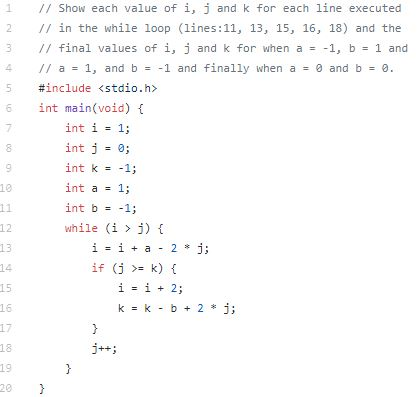
\includegraphics{debug.jpg}} 
\newpage 
\end{enumerate}
\end{document} 
